\documentclass[12pt]{article}
\usepackage{lecture}
\usepackage{graphicx}
\usepackage{html}
\usepackage{url}
\usepackage{epstopdf}

\newcommand{\copyrightYears}{2010--2021}

\title{Statistical phylogeography: Admixture graphs ans SPARG}

\begin{document}

\maketitle

\thispagestyle{first}

When I introduced the coalescent several weeks ago, I mentioned the
``Out of Africa'' hypothesis{\dash}the hypothesis that anatomically
modern humans evolved in Africa and spread from there throughout the
rest of the world. Three decades of research have strengthened support
for that hypothesis, and it is now widely accepted that anatomically
modern human populations left Africa and moved into other parts of the
world about 50,000 years ago~\cite{Karmin-etal-2015}. As they
expanded, they interacted with archaic human populations, e.g.,
Neanderthals and Denisovans. And when human populations interact,
interbreeding often occurs. The result is that 1-3 percent of human
genomes from outside of sub-Saharan Africa show evidence of
Neanderthal ancestry~\cite{Prufer-etal-2014} and that as much as 5 or
6 percent of the human genomes from Oceania show evidence of ancestry
from Denisovans~\cite{Meyer-etal-2012}. When we visualize these
relationships~(Figure~\ref{fig:human-neanderthal-denisovan}), the
result no longer looks like a simple tree. There are lines connecting
different branches representing times when there was some degree of
interbreeding among populations that had previously diverged. You may
have encountered methods for inferring phylogenies in previous
courses. In this course we saw how {\tt STRUCTURE} can be used to
estimate patterns of admixture. How do we go about estimating trees
that are admixed? Funny you should ask.

\begin{figure}
  \begin{center}
    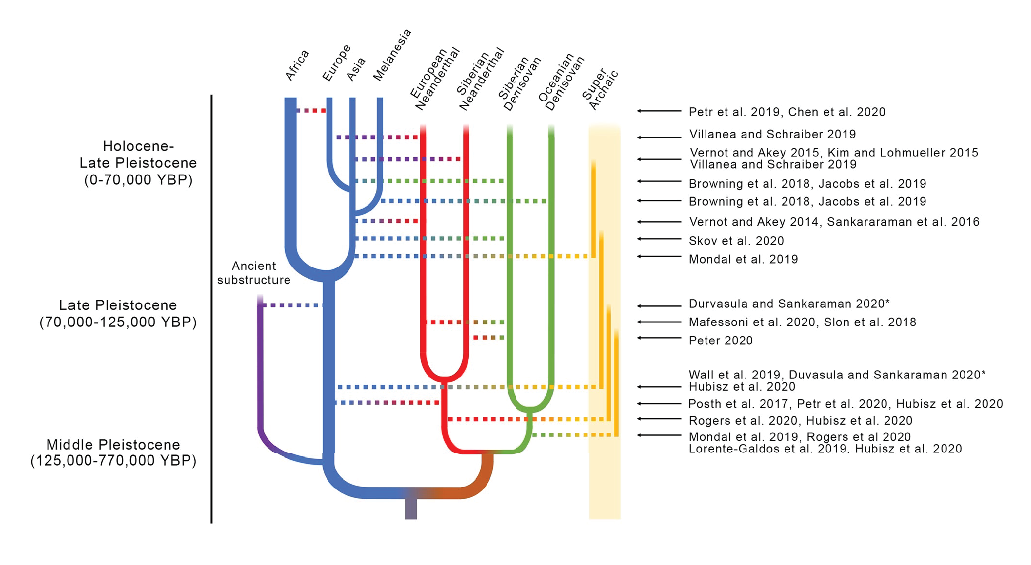
\includegraphics[width=14cm]{human-neanderthal-denisovan.eps}
  \end{center}
  \caption{Periods of introgression in humah
    history~(from~\cite{Ahlquist-etal-2021}).}\label{fig:human-neanderthal-denisovan}
\end{figure}

\section*{Admixture graphs}\index{admixture graphs}

Pickrell and Pritchard~\cite{Pickrell-Pritchard-2012} described the
most widely used approach to estimating admixture graphs. It is
implemented in {\tt TreeMix}.\index{TreeMix} At about the same time
Patterson et al.~\cite{Patterson-etal-2012} described a related method
at about the same time. I'm going to focus on the {\tt TreeMix}
approach because I am more comfortable with the underlying
model.\footnote{If you're curious about why I'm more comfortable with
  the Pickrell and Pritchard approach, feel free to ask.}
Unfortunately, if you want to use {\tt TreeMix}, you'll have to be comfortable
with compiling C++ programs from source~(or find a friend who can help
you or who can share a copy).\footnote{The most recent version of the
  {\tt TreeMix} manual notes that ``TreeMix should run on any Unix or
  Unix-like (e.g., Linux or Mac OS X) system. It may be more difficult
  to get it compiled under Windows. Notice that regardless of
  operating system, you'll also need to install the GNU Scientific
  Library and the Boost Graph Library.''}

The basic idea between {\tt Treemix} is not too complicated, although
it would be a stretch to say that it's simple. We start by assuming
that the allele frequencies are changing as a result of genetic
drift. Results going back to Kimura~\cite{Kimura-1955} tell us that
the variance in allele frequency is
\[
  \mbox{Var}(p_t) = p_o(1-p_0)\left(1 - e^{-t/2N_e}\right) \quad ,
\]
where $p_t$ is the allele frequency in the population at time $t$,
$p_o$ is the initial allele frequency, $t$ is the number of
generations, and $N_e$ is the effective population size. So long as
the effective population size is large enough that allele frequency
changes are relatively small from generation to generation and so long
as $p_o$ is not ``too close'' to 0 or 1, then we can approximate the
probability distribution of allele frequencies at time $t$ with a
normal distribution:
\[
  \mbox{P}(p_t|p_o,t,N_e) \sim \mbox{N}\left(p_o,
    p_o(1-p_o)\left(\frac{t}{2N_e}\right)\right) \quad .
\]
Now suppose we have a series of four populations related like those
shown in Figure~\ref{fig:treemix-no-migration}. As you can see, this
example shows populations that have a simple tree-like
relationship. Here's where the fun starts.

\begin{figure}
  \begin{center}
    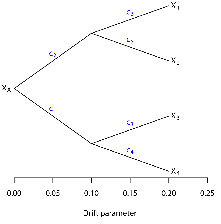
\includegraphics[width=12cm]{treemix-no-migration.eps}
  \end{center}
  \caption{A purely tree-like relationship among four hypothetical
    populations. The allele frequencies in each population are
    represented by $X_i$. The drift parameter on the $x$-axis is $t/2N_e$,
    i.e., it's measuring time from the root of the tree to the tips in
    units of $1/2N_e$. A part of a figure in~\cite{Pickrell-Pritchard-2012}.}\label{fig:treemix-no-migration}
\end{figure}

It's a well known fact~\cite{CavalliSforza-Edwards-1967} that the
variance in allele frequencies ($X_i$ in the figure) are simply
\begin{eqnarray*}
  \mbox{Var}(X_1) &=& (c_2 + c_6)X_A(1-X_A) \\
  \mbox{Var}(X_2) &=& (c_2 + c_5)X_A(1-X_A) \\
  \mbox{Var}(X_3) &=& (c_1 + c_3)X_A(1-X_A) \\
  \mbox{Var}(X_4) &=& (c_1 + c_4)X_A(1-X_A) \quad ,
\end{eqnarray*}
where $c_i = \frac{t_i}{2N_e^{(i)}}$, $t_i$ is the time associated
with branch $i$ and $N_e^{(i)}$ is the effective size of the
population associated with branch $i$. It's obvious from looking at
the tree that populations 1 and 2 have been evolving independently
from populations 3 and 4 from the start, while 1 and 2 have been
evolving independently of one another for a shorter period of time. As
a result, we expect allele frequencies in pouplations 1 and 2 to be
more similar than those in populations 3 and 4. In fact, Pickrell and
Pritchard point out that we can write the various covariances down
pretty simply too:
\begin{eqnarray*}
  \mbox{Cov}(X_1,X_2) &=& c_2X_A(1-X_A) \\
  \mbox{Cov}(X_1,X_3) &=& 0 \\
  \mbox{Cov}(X_1,X_4) &=& 0 \\
  \mbox{Cov}(X_2,X_3) &=& 0 \\
  \mbox{Cov}(X_2,X_4) &=& 0 \\
  \mbox{Cov}(X_3,X_4) &=& c_1X_A(1-X_A) \quad .
\end{eqnarray*}
As a result, we can write down a multivariate probability distribution
that describes all of the allele frequencies simultaneously, given the
same caveats as above about the normal distribution.
\[
  \mbox{P}(\bf p_t|\bf p_0, \bf t, \bf N_e) \sim \mbox{MVN}(\bf p_0,
  \bf \Sigma) \quad ,
\]
where boldface refers to vectors, MVN refers to the multivariate
normal distribution, and $\bf Sigma$ is the covariance matrix of
allele frequencies. Since we can write down that probability
distribution, you can probably imagine that it's possible to estimate
the likelihood of our data given a particular tree. To get a maximum
likelihood estimate of how our populations are related, assuming
there's no migration, we simply have to compare the likelihoods across
all possible trees and choose the one that's most likely.\footnote{If
  you know anything about estimating phylogenies, you know there is
  tremendous complexity buried in that ``simply have to compare.''
  Also notice that if we can get a maximum likelihood estimate, we can
  also get a full Bayesian posterior ``simply'' by providing the
  appropriate priors.}

Now suppose we allow migration from one of our populations into
another. The simple example Pickrell and Pritchard
provide~(Figure~\ref{fig:treemix-figure} shows a single migration from
the lineage leading to population 2 into population 3, labeling the
source population as $Y$ and the destination population as $Z$. As you
can see in Panel D of the figure, the migration event changes the
structure of the covariance matrix. Since all the migration event does
is to change the covariance matrix, we can once again explore
parameter space and find the network that maximizes the
likelihood. When we do so, not only do we have estimates for
population relationships and effective population sizes but also for
the timing and direction of migration events. Estimating admixture is,
however, even more challenging than estimating a population
phylogeny. The number of alternative configurations explodes rapidly
with more than 4-5 populations, making heuristic searches
necessary. Molloy et al.~\cite{Molloy-etal-2021} recently described a
new approach that builds on {\tt TreeMix} and seems to avoid getting
stuck in a local optimum. Since the basic approach is the same and
this isn't a course in computational biology, we won't discuss it
further, but you should investigate it if you use admixture graphs in
any of your work.

\begin{figure}
  \begin{center}
    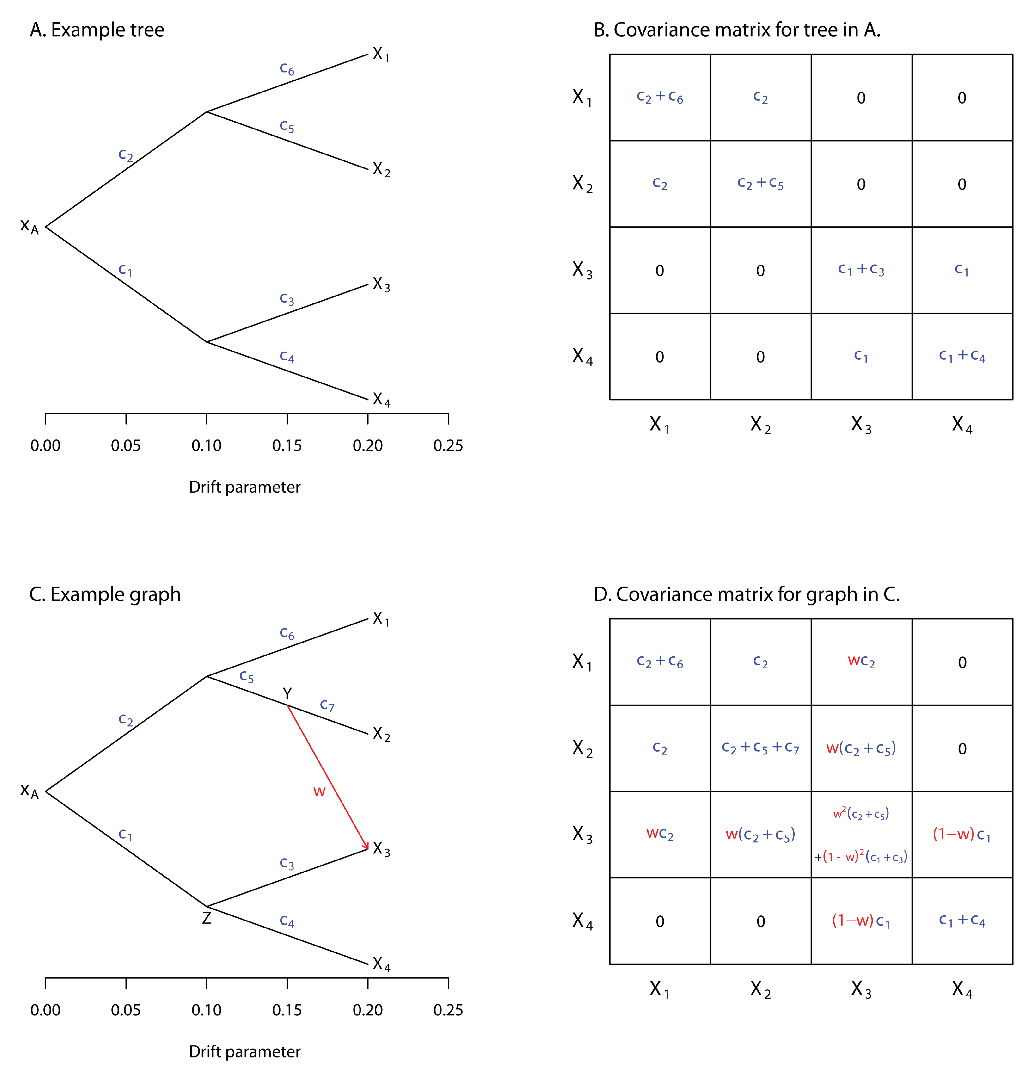
\includegraphics[width=12cm]{treemix-figure.eps}
  \end{center}
  \caption{Illustrating the covariance matrices of admixed and
    unadmixed populations. From \cite{Pickrell-Pritchard-2012}.}\label{fig:treemix-figure}
\end{figure}

\bibliography{popgen}
\bibliographystyle{plain}

\ccLicense

\end{document}


\bibliography{popgen}
\bibliographystyle{plain}

\ccLicense

\end{document}
